% A Theory section should extend, not repeat, the background to the
% article already dealt with in the Introduction and lay the
% foundation for further work.

% 13:45 Start. 15:00 End. 1h 15m total.

\section{Theoretical Background}
\label{sec: backg}

Here, we'll introduce some key concepts essential for grasping the foundations of this work.

% Something about the background goes here. Describe MaxCut and state-of-the-art: Goemans-Williamson (Classical), QAOA (Quantum-Classical) and QEMC (Classical, but quantum-inspired).

\subsection{Hybrid Quantum-Classical Computing}
\label{sec: HQCC}
Hybrid quantum-classical computing refers to a computational approach that combines elements of both classical and quantum computing paradigms to leverage the strengths of each. In this model, classical processors and quantum processors work in tandem to solve complex problems more efficiently than either could achieve alone. This collaborative strategy aims to harness quantum computing's unique capabilities while mitigating the challenges and limitations associated with quantum systems, such as error correction and decoherence. As of today, the synergy between classical and quantum elements holds promise for addressing complex real-world problems in areas like optimization, machine learning, and cryptography \cite{Cerezo_2021}.

\begin{figure*}[b]
    \centering
    \begin{equation}\label{eq:param_shift}\tag{3}
        \frac{\partial C}{\partial \theta_l} = \sum_k \frac{1}{2\sin{\alpha}}\left(Tr\left[O_k U(\boldsymbol{\theta_+}) \rho_k U^{\dagger}(\boldsymbol{\theta_+})\right] - Tr\left[O_k U(\boldsymbol{\theta_-}) \rho_k U^{\dagger}(\boldsymbol{\theta_-})\right]\right)
    \end{equation}
    % \caption{Parameter-shift rule equation.}
\end{figure*}

\subsubsection{Variational Quantum Algorithms}
The essence of HQCC lies in VQAs, which use parameterized quantum circuits (Ansätze). These algorithms employ classical optimization to adjust the quantum circuit parameters, similar to how neural networks are trained to minimize a cost function. This approach leverages classical optimization tools and keeps quantum circuit depth shallow, reducing noise and making VQAs suitable for the current NISQ era. VQAs have diverse applications and are considered the most promising avenue for achieving near-term quantum advantage, despite challenges in trainability, accuracy, and efficiency \cite{Cerezo_2021}.

The development of a VQA involves defining a cost function, \( C \), representing the problem's solution. Then, an ansatz, a parameterized quantum circuit, is proposed, with parameters \(\boldsymbol{\theta}\) to be optimized. The ansatz undergoes training in a hybrid quantum-classical loop to minimize \( C(\boldsymbol{\theta}) \) (Eq. \ref{eq:Optimization}). Quantum computation estimates \( C(\boldsymbol{\theta}) \) and its gradient, while classical routines optimize \(\boldsymbol{\theta}\). Further details for each step of the VQA framework are provided.

\begin{equation}\label{eq:Optimization}
\boldsymbol{\theta}^{\star} = \arg \min_{\boldsymbol{\theta}} C(\boldsymbol{\theta})
\end{equation}

\noindent {\bf \myFontSize Cost function:} Defining the VQA involves constructing a cost function that assigns numerical values to trainable parameters \(\boldsymbol{\theta}\). This function shapes a cost landscape for optimization. The aim is to identify its global minimum, representing the solution (Eq. \ref{eq:Optimization}). Typically, the cost takes the form of Eq. \ref{eq:Cost}, consisting of functions \(\{f_k\}\), a parameterized unitary \(U(\boldsymbol{\theta})\), input states \(\rho_k\), and observables \(O_k\). Oftentimes, it is convenient to design the cost function to be given by the expectation value of a Hamiltonian (e.g., the cost Hamiltonian in QAOA), which is why we mention that it is beneficial for it to have this specific form.
\begin{equation}\label{eq:Cost}
C(\boldsymbol{\theta}) = \sum_k f_k\left( Tr\left[O_k U(\boldsymbol{\theta}) \rho_k U^{\dagger}(\boldsymbol{\theta})\right] \right)
\end{equation}
% \\

% This last sentence can be removed, if space in required: "Ensuring the faithfulness and efficient estimation of \(C(\boldsymbol{\theta})\) are essential for successful VQA implementation, requiring experimental validation." Removed!

\noindent {\bf \myFontSize Ansatz:} The ansatz (parameterized quantum circuit) plays a crucial role in determining the parameters $\boldsymbol{\theta}$ and their optimization to minimize the cost. Ansatz design can be problem-inspired or agnostic, with each approach offering distinct advantages. Problem-agnostic Ansätze are versatile but may require more parameters, complicating optimization. In contrast, problem-oriented Ansätze incorporate problem-specific information, potentially reducing the parameter space and improving interpretability. Choosing between these approaches involves balancing accuracy and generality, considering resource utilization. While problem-inspired Ansätze often yield superior performance, their design presents challenges. Common ansatz types include hardware-efficient, unitary coupled clustered, and quantum alternating operator Ansätze, among others. \\

\noindent {\bf \myFontSize Gradients and training:} After defining the cost function and ansatz, the next step involves training the parameters \(\boldsymbol{\theta}\) to optimize Eq. \ref{eq:Optimization}. Analytically computing the gradient of the cost function is a notable advantage of many VQAs, achieved using the parameter-shift rule (Eq. \ref{eq:param_shift}), where \(\boldsymbol{\theta_{\pm}} = \boldsymbol{\theta} \pm \alpha \boldsymbol{e_l}\), holds for any real number \(\alpha\). Practically, \(\alpha = \pi/4\) is commonly used for accuracy \cite{Cerezo_2021}. The VQA workflow resembles traditional machine learning, with input states processed by an ansatz parameterized by \(\boldsymbol{\theta}\), followed by measurement and cost function estimation. A classical optimizer updates \(\boldsymbol{\theta}\) iteratively until convergence to find the optimal parameters \(\boldsymbol{\theta}^{\star}\). This high-level overview illustrates how VQAs function within a hybrid loop. Therefore, specifying the cost function and ansatz will be sufficient to characterize them.

% \begin{equation}\label{eq:Gradient}
% \frac{\partial C}{\partial \theta_l} = \sum_k \frac{1}{2\sin{\alpha}}\left(Tr\left[O_k U(\boldsymbol{\theta_+}) \rho_k U^{\dagger}(\boldsymbol{\theta_+})\right] - Tr\left[O_k U(\boldsymbol{\theta_-}) \rho_k U^{\dagger}(\boldsymbol{\theta_-})\right]\right),
% \end{equation}

\subsection{MaxCut Problem}
\label{sec: MaxCut}
The MaxCut problem, a fundamental problem in graph theory and combinatorial optimization, involves partitioning a graph \( G = (V, E) \) into two disjoint subsets, \( S_1 \) and \( S_2 \), such that the number of edges connecting vertices from different subsets is maximized. Formally, the objective is to find a partition \( (S_1, S_2) \) that maximizes:

\begin{equation}\label{eq:Cut}\tag{4}
\text{Cut}(S_1, S_2) = \sum_{(u, v) \in E} \chi(u, v),
\end{equation}
where \( \chi(u, v) = 1 \) if \( u \) and \( v \) belong to different subsets, and \( \chi(u, v) = 0 \) if they belong to the same subset. This quantity is referred to as the "cut" of the partition $(S_1, S_2)$. Pictorially, this can be represented as cutting the edges of the graph (Figure \ref{fig:MaxCut}), hence the name MaxCut. What we describe here is the un-directed, un-weighted MaxCut problem. A more general formulation would involve the specific graph's adjacency matrix, $W_{ij}$. % Can also remove this last part here: "What we describe here is the un-directed, un-weighted MaxCut problem. A more general formulation would involve the specific graph's adjacency matrix, $W_{ij}$."

Since the MaxCut problem is NP-hard, finding an optimal solution efficiently is a significant computational challenge, especially as the graph size grows. However, researchers have developed various approximation algorithms and heuristics to approach near-optimal solutions in a reasonable time, including both classical and quantum approaches. % These methods are designed to tackle the intrinsic complexity of the problem, providing practical solutions that have real-world applications. % As mentioned earlier, the MaxCut problem finds use in a variety of fields, including machine learning \cite{937505}, statistical physics \cite{Barahona_Grötschel_Jünger_Reinelt_1988}, circuit design \cite{Barahona_Grötschel_Jünger_Reinelt_1988}, and data clustering \cite{10.1007/11893318_21}.
 
% This last sentence can be removed, if space in required.

\begin{figure}[H]
  \centering
  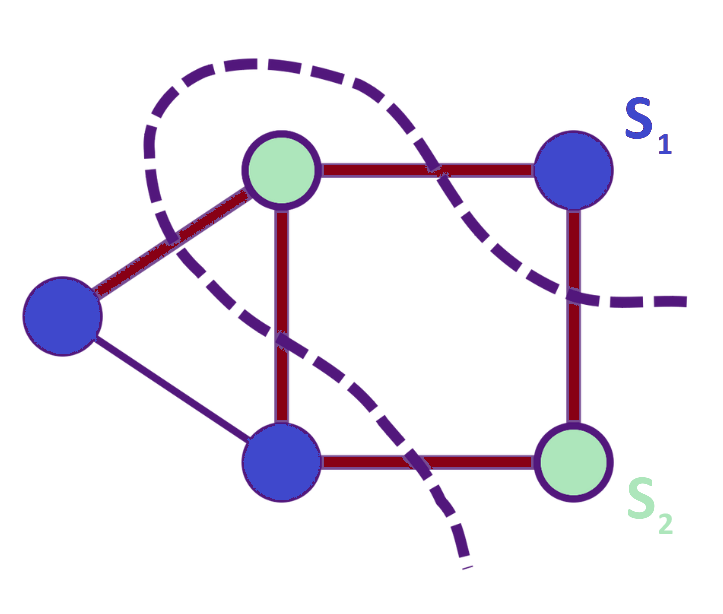
\includegraphics[width=0.95\columnwidth]{Figures/MaxCut.png}
  \caption{An example of a graph with a partition that maximizes the number of cut edges (red). Note that the MaxCut partition might not be unique.} % 'The number of edges that are cut is promptly labeled as the "cut".' Removed!
  \label{fig:MaxCut}
\end{figure}

\subsection{State-of-the-Art Algorithms}
\label{sec: SoA}
Next, we introduce the state-of-the-art algorithms for tackling the MaxCut problem, encompassing both classical (Goemans-Williamson) and hybrid quantum-classical (QAOA and QEMC) approaches.

% QAOA Ansatz image. It's here because of the weird rules that govern figure positioning in LaTeX.
\begin{figure*}[b]
  \centering
  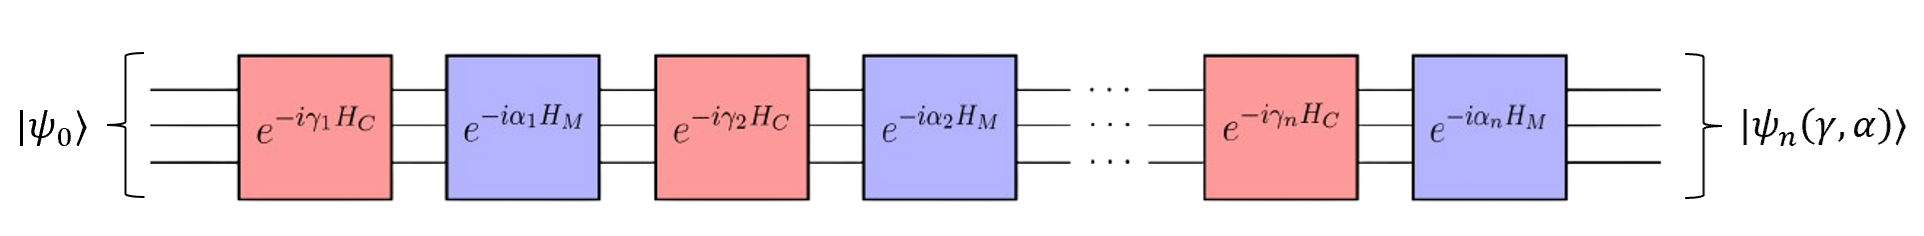
\includegraphics[width = \textwidth]{Figures/QAOA_Trotterization.png}
  \caption{Quantum alternating operator ansatz. Adapted from \cite{Intro_QAOA}.}
  \label{fig:QAOA_Trotterization}
\end{figure*}

\subsubsection{Goemans-Williamson Algorithm}
\label{sec: GW}
%In this section, we explore the Goemans-Williamson (GW) Algorithm, pivotal in combinatorial optimization, especially for MaxCut.

Developed by Goemans and Williamson in 1995, this algorithm employs semidefinite programming to create an approximate solution, later refined for a near-optimal cut. Semidefinite programming optimizes a linear function over a symmetric matrix while ensuring positive semidefiniteness. It finds applications in control theory, nonlinear programming, geometry, and combinatorial optimization, as detailed in \cite{GW-Algorithm} and references therein.

% This can be removed too: "It finds applications in control theory, nonlinear programming, geometry, and combinatorial optimization, as detailed in \cite{GW-Algorithm} and related references."

The Goemans-Williamson algorithm addresses the MaxCut problem through a series of mathematical formulations and randomized procedures. Initially, an integer quadratic program \( (Q) \) is defined to maximize the "cut" in a graph. This is represented by binary variables \( y_i \), where \( S_1 \) and \( S_2 \) correspond to the vertices with values $1$ and $-1$, respectively. However, since solving \( (Q) \) directly is NP-hard, the algorithm instead employs a semidefinite programming relaxation \( (P) \), which relaxes constraints to optimize vectors \( v_i \in S_n \) rather than \( y_i \). This relaxation is represented as:
\begin{equation}\tag{5}
    \begin{aligned}
        &\text{Maximize}\;\;\frac{1}{2}\sum_{\substack{i < j: \\ (i,j)\in E}}(1-v_{i} \cdot v_{j}) \\
        (P)\qquad&\text{Subject to: }v_{i}\in S_n \qquad\forall i\in V,
    \end{aligned}
\end{equation}
where \( v_i \) are vectors constrained to the \( n \)-dimensional unit sphere ($S_n$). The algorithm then proceeds as follows:
\begin{enumerate}
    \item Solve \( (P) \) to obtain optimal vectors \( v_i \);
    \item Select a random vector \( r \) uniformly distributed on $S_n$;
    \item Partition vertices into \( S_1 \) and \( S_2 \) based on whether \( v_i \cdot r \geq 0 \) or \( v_i \cdot r < 0 \).
\end{enumerate}
Effectively, the algorithm divides vertices based on a randomly chosen hyperplane in \( n \) dimensions. The performance guarantee of the Goemans-Williamson algorithm is quantified by the approximation ratio \( \alpha > 0.878 \) \cite{GW-Algorithm}.

%%%%%%%% Separating the two options %%%%%%%%
%%%%%%% This is what I had written before: %
%%% Now, I've cut it short, to have more %%%
%%%%%% space for the other sections. %%%%%%%

% Formally, the Goemans-Williamson algorithm can be described as follows \cite{GW-Algorithm}. Given a graph with vertex set \( V = \{1, ..., n\} \) and non-negative weights \( w_{ij} = w_{ji} \) for each pair of vertices \( i \) and \( j \), the weight of the maximum cut \( w(S_1, S_2) \) is obtained from the integer quadratic program:
% I wonder if I should mention that this formulation is entirely equivalent to the previous expression, with \Chi. If I have space, at the end of this, I guess I can add this.
% \begin{equation}
%     \begin{aligned}\label{eq:GW_Q}
%       &\text{Maximize}\;\;\frac{1}{2}\sum_{\substack{i < j: \\ (i,j)\in E}}w_{i j}(1-y_{i}y_{j}) \\
%       (Q)\qquad&\text{Subject to: }y_{i}\in\{-1,1\}\qquad\forall i\in V,
%     \end{aligned}
% \end{equation}
% where \( S_1 = \{i \mid y_i = 1\} \) and \( S_2 = \{i \mid y_i = -1\} \) correspond to a cut of weight
% \begin{equation}
% w(S_1, S_2) = \frac{1}{2} \sum_{\substack{i < j \\ (i,j) \in E}} w_{ij} \left(1 - y_i y_j\right).
% \end{equation}
% Solving this NP-hard program with the GW algorithm involves relaxing constraints, resulting in a semidefinite programming relaxation \((P)\):
% \begin{equation}
%     \begin{aligned}
%       &\text{Maximize}\;\;\frac{1}{2}\sum_{\substack{i < j: \\ (i,j)\in E}}w_{i j}(1-v_{i} \cdot v_{j}) \\
%       (P)\qquad&\text{Subject to: }v_{i}\in S_n \qquad\forall i\in V.
%     \end{aligned}
%     \end{equation}    
% The GW algorithm then proceeds as follows:
% \begin{enumerate}
%   \item Solve \((P)\) to obtain optimal vectors \( v_{i} \);
%   \item Select a random vector \( r \) uniformly distributed on \( S_n \) ($n$-dimensional unit sphere);
%   \item Partition vertices into \( S_1 \) and \( S_2 \) based on whether \( v_{i} \cdot r \geq 0 \) or \( v_{i} \cdot r < 0 \).
% \end{enumerate}
% This method essentially partitions vertices based on a randomly chosen hyperplane in \( n \) dimensions, dividing them into \( S_1 \) and \( S_2 \) accordingly. Furthermore, it can be shown that the GW algorithm has a performance guarantee of:
% \begin{equation}
%   \alpha=\operatorname*{min}_{0\,\leq\,\theta\leq\pi}\,\frac{2}{\pi}\,\frac{\theta}{1\,-\,\cos\,\theta} > \,0.878.
% \end{equation}
% A comprehensive proof outlining the derivation of this $0.878$ value is available in section $3$ of \cite{GW-Algorithm}, along with a more in-depth exposition of the algorithm.

% I should, at some point, say that I present these state-of-the-art algorithms to provide a benchmark for the iQAQE algorithm. This is important to show that the iQAQE algorithm is competitive with the best algorithms available.

\subsubsection{Quantum Approximate Optimization Algorithm (QAOA)}
\label{sec: QAOA}
% In accordance with the previous section, it suffices to present the QAOA cost function and ansatz to fully characterize it.
% Define the cost as the expectation value of the so-called cost/problem Hamiltonian. Present the form of this Hamiltonian and explain why it works (interpretation, essentially).
% Then, present the Trotter-inspired ansatz: the Quantum Alternating Operator Ansatz. Put the image and explain what the blocks means: cost/problem Hamiltonian and mixer/bias Hamiltonians' complex exponentials. Present these Hamiltonians' forms and their complex exponentials' circuit implementation.
% Also, mention that the uniform superposition enters the ansatz, and the partition is decided by the most frequently sampled basis state, at the end of the circuit, after training.

The QAOA, renowned for its prowess in quantum-enhanced optimization, was initially crafted to tackle a range of combinatorial optimization problems such as constraint-satisfaction \cite{lin2016performance} and MaxCut \cite{PhysRevA.97.022304}. QAOA utilizes a cost Hamiltonian, denoted as \(H_C\), which serves as the basis for extracting the objective function. This Hamiltonian is formed by associating each conventional classical variable $y_i$ with a Pauli spin \(1/2\) operator, represented as \(\boldsymbol{Z}_j\). Formally, the usual MaxCut objective $L(y) = \frac{1}{2}\sum_{\substack{i < j: \\ (i,j)\in E}}(1-y_{i}y_{j})$, denoting the cut of partition $y = (y_1,...,y_N)$, is transformed into the cost Hamiltonian
\begin{equation}\label{eq:H_C}\tag{6}
  H_C = \frac{1}{2}\sum_{\stackrel{i < j:}{(i,j)\in E}}(1-\boldsymbol{Z}_i\boldsymbol{Z}_j).
\end{equation}

The Trotter-inspired QAOA ansatz involves $n$ cycles of alternating time evolution between $H_C$ and a mixer Hamiltonian, $H_M$. The role of this mixer Hamiltonian can be understood as introducing quantum fluctuations, or transitions, between different states, helping the algorithm explore the solution space more effectively, ideally preventing it from getting trapped in sub-optimal local minima. This ansatz, depicted in Figure \ref{fig:QAOA_Trotterization}, illustrates $n$ QAOA layers, each comprising alternating applications of $H_C$ and $H_M$. 

The cost function \(C(\boldsymbol{\gamma}, \boldsymbol{\alpha})\) is determined by the expectation value of \(H_C\) over the ansatz state \(\ket{\psi_n(\boldsymbol{\gamma}, \boldsymbol{\alpha})}\), obtained at the end of the quantum circuit (Figure \ref{fig:QAOA_Trotterization}). In practice, defining $\boldsymbol{\theta} = \{\boldsymbol{\gamma}, \boldsymbol{\alpha}\}$, the cost function is $C(\boldsymbol{\gamma}, \boldsymbol{\alpha}) = \bra{\psi_n(\boldsymbol{\gamma}, \boldsymbol{\alpha})}H_C\ket{\psi_n(\boldsymbol{\gamma}, \boldsymbol{\alpha})}$, with
\begin{equation}\label{eq:QAOA_ansatz}\tag{7}
    \scalebox{0.825}{$\displaystyle
    \ket{\psi_n(\boldsymbol{\gamma}, \boldsymbol{\alpha})} = e^{-i\alpha_nH_M}e^{-i\gamma_nH_C} ... e^{-i\alpha_1H_M}e^{-i\gamma_1H_C}\ket{\psi_0},$}
\end{equation}
where $\ket{\psi_0}$ is the initial state entering the ansatz. In QAOA, it is customary to start with a uniform superposition over the $N$ bit-string\footnote{Keep in mind, there's one qubit allocated for each graph node.} basis states, i.e., $\ket{\psi_0} = \ket{+}^{\otimes N}=\frac{1}{\sqrt{2^{N}}}\sum_{z\in\{0,1\}^{N}}\ket{z}$. This is achieved by applying a Hadamard gate to each of the qubits, at the start of the quantum circuit.

In practice, the mixer Hamiltonian terms $e^{-i\alpha_l H_M}$ correspond to $R_x(2\alpha_l)$ and are easy to implement. The cost Hamiltonian terms, on the other hand, are a bit more tricky, requiring the use of $2$ CNOT gates. Each of the terms $e^{-i\gamma_l(1-\boldsymbol{Z}_{j}\boldsymbol{Z}_{k})/2}$ can be transpiled into a quantum circuit, as shown in Figure \ref{fig:Z_iZ_jDecomposition}. For each edge in the graph, we'll have one of these terms, in each of the $n$ layers of the QAOA ansatz.
\begin{figure}[H]
  \centering
  \begin{quantikz}
  \lstick{Qubit $i$} & \ctrl{1} & \qw                & \ctrl{1}  & \qw & \\
  \lstick{Qubit $j$} & \targ{}  & \gate{R_z(\gamma_l)} & \targ{}   & \qw & \\
  \end{quantikz}
  \caption{$e^{i\gamma_l \boldsymbol{Z}_{i} \boldsymbol{Z}_{j} /2}$ decomposition.}\label{fig:Z_iZ_jDecomposition}
\end{figure}

Subsequently, a classical routine is employed to optimize the values of the parameters by minimizing the negative of the cost (analogous to the "cut"), therefore enabling the extraction of the MaxCut partition.

\begin{figure*}[b]
  \centering
  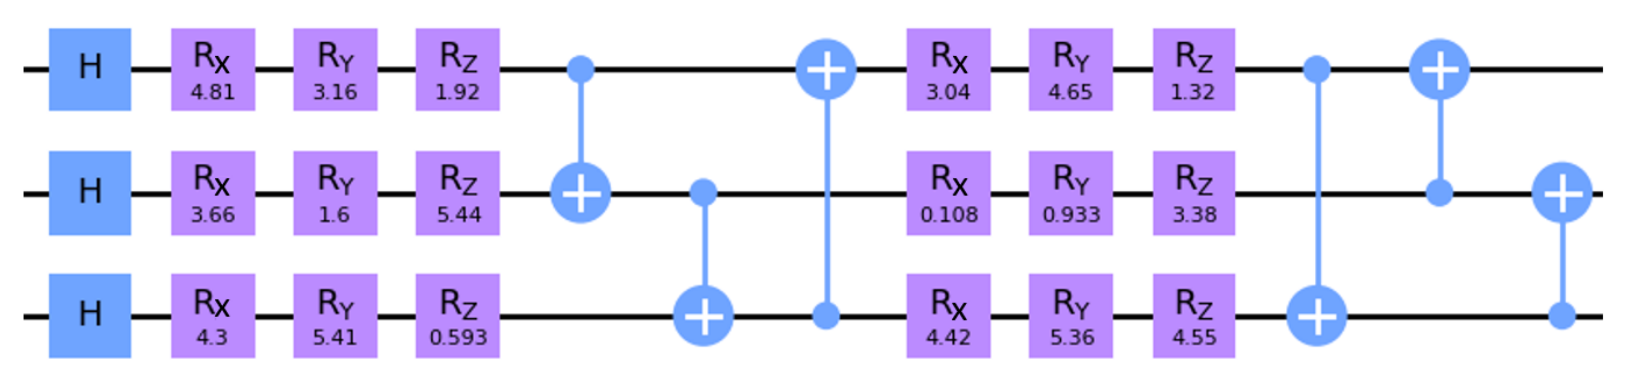
\includegraphics[width = \textwidth]{Figures/Strongly_Entangling_Layers.png}
  \caption{"Strongly Entangling Layers" circuit ansatz: case of $n = 3$ qubits and $p = 2$ layers. After a single layer of Hadamard gates, each subsequent layer consists of $3n$ single-qubit parameterized rotation gates and $n$ CNOT gates (entangling gates). Reproduced from \cite{tenecohen2023variational}.}
  \label{fig:Strongly_Entangling_Layers}
\end{figure*}

\subsubsection{Qubit-Efficient MaxCut Heuristic Algorithm (QEMC)}
\label{sec: QEMC}
% Just summarize the thesis's section on this.

QEMC \cite{tenecohen2023variational} is somewhat similar to QAOA. However, it has a number of crucial differences. First, it only requires $n = \log_2(N)$ qubits, instead of $N$, where $N$ is the number of nodes in the graph. Additionally, the QEMC algorithm is based on a novel probability threshold encoding scheme, a suitable cost function, and a parameterized unconstrained quantum circuit. Going in order: \vspace{1.5mm}

\noindent {\bf \myFontSize Probability threshold encoding scheme:} With $n$ qubits, each of the $N = 2^{n}$ basis states will represent one of the graph's nodes. Following the sampling of the quantum circuit, a probability distribution is generated. Nodes with probabilities exceeding a certain threshold, $p_{th} = \frac{1}{2B}$, belong to "Set 1", while probabilities below this value indicate inclusion in "Set 0". This strongly diverges from how we encode set inclusion in QAOA. \\

\noindent {\bf \myFontSize Cost function:} The objective function utilized in QEMC is the following:

\begin{equation}\tag{8}
    \scalebox{0.75}{$\displaystyle
    L(\{p(i)\}) = \sum_{\stackrel{j < k:}{(j,k)\in E}}\left[\left(d(j,k)-\frac{1}{B}\right)^{2}+\left(s(j,k)-\frac{1}{B}\right)^{2}\right],$}
\end{equation}
where $d(j,k) = |p(j) - p(k)|$ and $s(j, k) = p(j) + p(k)$ are the absolute difference and sum of the corresponding states' probabilities. The idea is that as both $d(j, k)$ and $s(j, k)$ tend towards $1/B$, the probability of one node approaches zero (distinctive "Set 0"), while the probability of the other node approaches $1/B$ (distinctive "Set 1"), without specifying which is which. Ultimately, just like for QAOA, connections between nodes of different sets are favoured. Note, however, that this probability threshold encoding scheme assumes \textit{a priori} that one of the sets ("Set 1") has $B$ nodes. Nevertheless, this is not an issue, as we can efficiently iterate through all potential values of $B\,=\,1,...,\left\lfloor{\frac{N}{2}}\right\rfloor$. Frequently, it is reasonable to set $B = N/2$, and we shall use this as our default starting point. \\

\noindent {\bf \myFontSize Problem-agnostic ansatz:} The QEMC circuit ansatz is agnostic to specific graph instances, a departure from QAOA where the graph structure is explicitly encoded in the quantum circuit. Instead, the graph is implicitly encoded through the cost function. As a result, the QEMC quantum circuit is not bound to any particular form and only needs to be expressive enough to approximate the optimal states in the Hilbert space. Such problem-independent ansatz approach provides considerable flexibility in ansatz selection. Frequently, the circuit ansatz known as "Strongly Entangling Layers" is employed, as depicted in Figure \ref{fig:Strongly_Entangling_Layers}. As can be seen, this ansatz applies a series of parameterized single-qubit rotations interspersed with entangling gates to generate a highly entangled quantum state. % We use PennyLane's \href{https://docs.pennylane.ai/en/stable/code/api/pennylane.StronglyEntanglingLayers.html}{\texttt{qml.StronglyEntanglingLayers}} implementation for this purpose.

% Can, maybe, remove "As can be seen, this ansatz applies a series of parameterized single-qubit rotations interspersed with controlled entangling gates to generate a highly entangled quantum state. We use PennyLane's \href{https://docs.pennylane.ai/en/stable/code/api/pennylane.StronglyEntanglingLayers.html}{\texttt{qml.StronglyEntanglingLayers}} implementation for this purpose."

% These constitute the main ingredients necessary to understand the QEMC algorithm. At this point, the same hybrid loop as before would be run, so as to optimize the "Strongly Entangling Layers" ansatz's parameters, to minimize the cost function. To read the MaxCut partition, generated by the QEMC algorithm, one would sample the circuit's output one more time, after the training, and build the basis states' probability distribution. The threshold $p_{th}$ would then be applied to determine each nodes' set inclusion, from each of their associated basis states' probabilities.

One notable, and perhaps unfortunate, property of QEMC is that it is efficiently simulable classically. Due to the exponential compression of the number of qubits, the algorithm can be feasibly simulated on a classical computer, even for large graphs, hence defeating its purpose as a quantum algorithm. This is something the authors of the algorithm \cite{tenecohen2023variational} realized in hindsight. For this reason, it is now termed a quantum-inspired classical algorithm.

% For the iQAQE Framework, maybe present the Table?

